\documentclass[sigconf,techreport]{acmart}

\usepackage[utf8]{inputenc}
\usepackage{url}
\usepackage{color,fancyvrb}
\usepackage{algorithm}
\usepackage{algpseudocode}
\usepackage{mathtools}

\usepackage[frozencache,cachedir=minted]{minted}
% \usepackage[finalizecache,cachedir=minted]{minted}
%\usepackage{minted}
\renewcommand{\MintedPygmentize}{./scripts/pygmentize.py}
\newlength{\mintednumbersep}
\AtBeginDocument{%
  \sbox0{\tiny00}%
  \setlength\mintednumbersep{\parindent}%
  \addtolength\mintednumbersep{-\wd0}%
}

\newenvironment{longlisting}{\captionsetup{type=listing}}{}
%\usepackage[skip=2pt]{caption} % example skip set to 2pt
\setlength{\belowcaptionskip}{10pt plus 3pt minus 2pt} % Chosen fairly arbitrarily
\setlength{\abovecaptionskip}{10pt plus 3pt minus 2pt} % Chosen fairly arbitrarily

\setminted{
	% linenos=true,
	autogobble,
	breaklines,
	tabsize=2,
	fontsize=\footnotesize,
	encoding=utf8,
	frame=lines,
	fontfamily=zi4,
	highlightcolor=green
}
\usepackage{etoolbox,xpatch}

\makeatletter
\AtBeginEnvironment{minted}{\dontdofcolorbox}
\def\dontdofcolorbox{\renewcommand\fcolorbox[4][]{##4}}
\xpatchcmd{\inputminted}{\minted@fvset}{\minted@fvset\dontdofcolorbox}{}{}
\xpatchcmd{\mintinline}{\minted@fvset}{\minted@fvset\dontdofcolorbox}{}{} % see https://tex.stackexchange.com/a/401250/
\makeatother

\setcopyright{acmlicensed}
\acmDOI{00.000/000_0}
\acmISBN{000-0000-00-000/00/00}
\acmConference[ABC '00]{A Boilerplate Conference}{January 0000}{Norfolk, Virginia, USA}
\acmYear{0000}
\copyrightyear{0000}
\acmPrice{0.00}

% When "techreport" class parameter is supplied:
%   * hide reference block from the front page
%   * hide copyright note from the front page
%   * change conference info in the header of alternate pages to title
%   * add page number in the center of the footer of non-title pages
\makeatletter
\@ifclasswith{acmart}{techreport}{
	\settopmatter{printacmref=false}
	\renewcommand\footnotetextcopyrightpermission[1]{}
	\fancyhead{}
	\fancyfoot{}
	\fancyhead[L]{\shorttitle}
	\fancyhead[R]{\shortauthors}
	\fancyfoot[C]{\thepage}
	% \AtBeginDocument{The pagesize is \texttt{a5paper}.\par}
}{}
\makeatother

\usepackage{xcolor}
\newcommand\crule[3][black]{\textcolor{#1}{\rule{#2}{#3}}}

\newcommand{\inlinemlir}[1]{\mintinline{mlir}{#1}}
\newcommand{\inlinepython}[1]{\mintinline{python}{#1}}
\newcommand{\inlinev}[1]{\mintinline{verilog}{#1}}

\usepackage{soul}
\sethlcolor{green}

\newif\iffinal
\finalfalse


\iffinal
	\newcommand{\maxx}[1]{}
	\newcommand{\ryan}[1]{}
	\newcommand{\kyle}[1]{}
	\newcommand{\ian}[1]{}
	\newcommand{\arham}[1]{}
	\newcommand{\commnt}[2]{#2}
\else
	\newcommand{\maxx}[1]{{\textcolor{red}{ Max: #1 }}}
	\newcommand{\ryan}[1]{{\textcolor{magenta}{ Ryan: #1 }}}
	\newcommand{\kyle}[1]{{\textcolor{yellow}{ Kyle: #1 }}}
	\newcommand{\ian}[1]{{\textcolor{orange}{ Ian: #1 }}}
	\newcommand{\arham}[1]{{\textcolor{pink}{ Arham: #1 }}}
	\newcommand{\commnt}[2]{{{\color{green} \{#1\}} {\color{blue} #2}}}
\fi


\begin{document}

\title{BraggHLS}


\author{Maksim Levental, Arham, Kaz, Ryan "the champ", Kyle, and Ian Foster}
\affiliation{%
	\institution{University of Chicago}
	\department{Department of Computer Science}
	\city{Chicago}
	\state{Illinois}
	\postcode{60637}
	\country{USA}
}
\email{{mlevental,..,foster}@uchicago.edu}

\renewcommand{\shortauthors}{Levental et al.}


\begin{abstract}
	In many experiment-driven scientific domains, such as high-energy physics and X-ray crystallography, high sample rates necessitate low latency near-sensor data processing.
	%\ian{Next text seems to me to be unnecessarily complicated. Maybe the logic can be: 1) ``Deep neural network (DNN) methods can enable efficient implementations of key data processing tasks; }
	Thanks to a recent profusion in high-level frameworks, and example models, Deep Neural Network (DNN) models have been investigated for such use cases.
	Despite such investigations, few DNNs have been deployed in practice, owing to the inability of deployment targets (hardware accelerators) to meet hard latency and collocation constraints.
	Here we present a case-study of translating/deploying a particular X-ray crystallography DNN model to an alternative platform, namely Field Programmable Gate Arrays.
	We discuss some of the currently available workflows, toolchains, and their advantages and disadvantages.
	Further we discuss an application specific design methodology (specific to this model) to general purpose tools.
	Our approach achieves lower latency than any of the alternatives at the cost of generalizability, achieving \commnt{TBD}{3µs/333KHz}.
	Finally, we discuss extensions to our methodology that would enable generalization without any sacrifice in performance.
\end{abstract}


%    \begin{CCSXML}
%    <ccs2012>
%    <concept>
%    <concept_id>
%        10002951.10003227.10003392</concept_id>
%        <concept_desc>Information systems~Digital libraries and archives</concept_desc>
%        <concept_significance>500</concept_significance>
%        </concept>
%        <concept>
%        <concept_id>10002951.10003260</concept_id>
%        <concept_desc>Information systems~World Wide Web</concept_desc>
%        <concept_significance>500</concept_significance>
%        </concept>
%        </ccs2012>
%    \end{CCSXML}

\ccsdesc[500]{Information systems~Digital libraries and archives}
\ccsdesc[500]{Information systems~World Wide Web}

% Comment the above block out to hide CCS Concepts or update as per https://dl.acm.org/ccs/ccs.cfm


\keywords{Memento, Web Archiving, Frogs}


\maketitle

\tableofcontents

\section{Introduction}\label{sec:introduction}
Certain areas of science perform experiments that achieve extremely high data rates; well known examples in high-energy physics are the CMS and ATLAS experiments at the LHC, which observe new collision events every 25ns and must report detection \commnt{\url{https://indico.cern.ch/event/395374/contributions/939905/attachments/1185975/1719379/20151113_RealTimeAnalysisLHC-4.pdf}}{of interesting events at upto 1MHz} (LHCb).
\commnt{more examples}{Similarly, }X-ray crystallography employs high-energy diffraction microscopy techniques, which can sample \commnt{\url{https://aip.scitation.org/doi/10.1063/5.0006531}}{at up to 1MHz}.
Such high data rate experiments face the challenge of either processing the data in-situ (colocal with the scientific apparatus) or buffering/caching for later retrieval and post-processing.
Case in point, if CMS and ATLAS were to capture all collision events, they would produce approximately 40 terabytes of data \commnt{\url{https://www.sciencedirect.com/science/article/pii/S2352711020303320}}{each second}.
Thus, any improvement in the real-time, near-sensor, processing capabilities, for operations such as filtering and triggering, of such experiment infrastructure can dramatically reduce the burden on downstream infrastructure and compute, in addition to accelerating the pace of experiment design and scientific discovery.

Deep Neural Networks, effective in many other academic and commercial domains, have recently been considered for \commnt{cite the physical review letters paper from hls4ml}{these real-time scientific use cases}.
For example, BraggNN, a DNN aimed at identifying Bragg diffraction peaks with high precision, has been shown to make peak position determinations with high accuracy.
Still, as of yet DNN models have not seen wide adoption in this area.
This is due to the limitations imposed by the hardware platforms on which they can typically be deployed - GPUs and other such DNN accelerators.
Primarily, such accelerators do not meet the hard real-time latency constraints, and secondarily they cannot be easily colocated with complex sensing apparatuses.
BraggNN, despite having been shown to have high speedup over the classical pseudo-Voigt peak fitting methods, making determinations in approximately 700µs, still falls short of the 1µs target for handling 1MHz sampling rates.
In addition, the current implementation of BraggNN, deployed to either a datacenter class GPU such as a NVIDIA V100, or even a workstation class GPU such as a NVIDIA RTX 2080Ti, has no practicable means to being deployed at the edge, i.e., adjacent or proximal to the high energy microscopy equipment.

Application Specific Integrated Circuits (ASIC) and Field Programmable Gate Arrays (FPGA) are alternative potential deployment targets for the kinds of processing techniques necessary for low latency scientific use cases.
To wit: the LHC currently uses a combination of ASICs and FPGAs for their Level-1 filtering system, which must process each sample within 25ns and make its decision (regarding filtering) within approximately 10 µs, the time represented by the amount of available buffering.
But ASICs and FPGAs are not a \commnt{haha.}{free lunch}.
ASICs, while offering the absolute lowest possible latency, in the smallest possible package, incur extremely high development costs, due to the complexity of the digital design process and the overall costs of fabrication.
FPGAs, present an intermediate along dimensions of cost, latency, and development complexity; at the cost of 20x larger area consumption, \commnt{how to cite that epfl page? find this stat in one of their papers?}{4x longer latency, and 12x higher power consumption} (relative to ASICs), they come with the added benefit, in the context of DNNs, of reconfigurability.
That is to say, a DNN deployed to an FPGA can be redeployed, reconfigured, and reparameterized an arbitrary number of times, whereas an ASIC is for all intents and purposes \commnt{overused already here but yea frozen isn\'t a good word}{frozen}.

One of the principle challenges in deploying DNNs to FPGAs and ASICs is translating the high-level (with respect to abstraction) representations that DNNs are typically represented as, to the Register Transfer Level (RTL) representations which can be used for FPGA and ASIC design.
The fundamental reason for the difficulty in performing this translation is most (if not all) DNN implementations presume some underlying compute architecture, while FPGAs and ASICs are, in effect, blank canvases (with respect to architecture).
Thus, deploying to FPGA and ASICs entails reimagining a DNN model as compute architecture unto itself, including sophisticated considerations such as operation scheduling, register pipelining, and wire delay.
For conventional use-cases of FPGAs and ASIC, the development methodology involves an enormous \commnt{cite for clarify}{amount of hand-written or "hand-generated"} design of the primitive components (adders, multipliers, buses, etc.), a methodology dramatically distinct from conventional software design in general, and DNN design in particular.
Recently, though, with the advent of advanced compiler technologies, such as MLIR, and supported by advanced High-Level Synthesis (HLS) tools, it has become possible to practice an iterative design methodology that can in fact produce high-fidelity performant RTL representations of DNN models.

Thus, this work investigates the techniques and tools currently available for deploying DNNs to FPGAs.
Specifically, we deploy BraggNN to FPGA by performing a series of progressive \emph{lowerings} starting from a high-level representation (a PyTorch model) and culminating in synthesizable RTL (i.e., a representation that can be directly mapped to FPGA hardware).
Our work includes a survey of existing general purpose tools aimed at performing such lowerings, as well as our own \commnt{not really novel}{novel} approach.
We show that under certain assumptions, our approach produces inference latencies lower than that of any of the existing tools, achieving a peak end-to-end latency of 3µs/333KHz.
This latency represents a 200x improvement over the GPU implementation of BraggNN and only a 3x gap from the ultimate 1µs/1MHz latency target.

\commnt{A list of contributions is a nice clear way to say what youve done; shot fired - what have i contributed when you really think about it? i\'ll have to conjure some up}{The primary contributions of this paper are:}

\begin{enumerate}
	\item
\end{enumerate}
The remainder of this article is structured as such:
\begin{enumerate}
	\item Background on TS/MLIR, HLS, and logic synthesis;
	\item The challenges faced in using existing flows and how our approach addresses those challenges;
	\item An evaluation of our approach, as compared to existing tools, in terms of latency, resource usage, and development time;
	\item High priority goals, as we see them, for making this flow more ergonomic.
\end{enumerate}




\section{Background}\label{sec:background}
\subsection{BraggNN}\label{subsec:braggnn}

TODO: stuff about BraggNN

\subsection{Translating DNNs}\label{subsec:translatingdnns}
Our design methodology for BraggNN winds its way through several levels of abstraction and tooling:

\begin{enumerate}
	\item A conventional PyTorch representation;
	\item A JIT traced representation called TorchScript;
	\item Several, successively lower-level, MLIR representations;
	\item A LLVM IR representation;
	\item A RTL representation.
\end{enumerate}

We quickly review the relevant concepts of each level of abstraction.

\subsubsection{PyTorch/TorchScript}\label{subsec:pytorch}

Typically DNN models are represented in terms of high-level frameworks implemented within general purpose programming languages.
Such frameworks are widely used because of their ease of use and large library of example implementations of various DNN model architectures.
Two such frameworks are TensorFlow and PyTorch.
BraggNN is implemented within PyTorch.
DNNs are developed within PyTorch using the \emph{define-by-run} methodology (also known as \emph{eager mode}).
Using this methodology, the developer writes conventional Python code that describes the sequential execution of the high-level operations comprising the model, and the dataflow graph (for purposes of backprop/autodiff) is simultaneously defined and constructed at runtime.
With respect to the developer, define-by-run, which is not unique to PyTorch, enables fast iteration at development time, at the cost of some runtime performance (when compared with frameworks that require statically specifying the model).

With respect to the kind of program analysis necessitated by our translation of BraggNN, there is another cost to define-by-run DNN specification: the dataflow graph (DFG) is never fully materialized\footnote{``...instead, every intermediate result records only the subset of the computation graph that was relevant to their computation.''~\cite{paszke2017automatic}} and the control flow graph (CFG) is difficult to extract from the semantics of the general purpose language (Python in the case of PyTorch).
The PyTorch organization, having recognized these issues (in the course and context of their own deployment projects), in recent years has implemented a Single Static Assignment (SSA) intermediate representation (IR), called TorchScript (TS) and concomitant tracing mechanism (colloquially referred to as the TS JIT compiler) to produce TS from conventionally defined PyTorch models.
The exact operation of this tracing mechanism is beyond the scope of our work\footnote{\url{https://github.com/pytorch/pytorch/wiki/PyTorch-dispatcher-walkthrough}}, but two of its limitations, as they pertain to our work, merit discussion.
Firstly, much like other JIT compilers, the TS JIT does not easily support control flow \footnote{(\inlinemlir{prim::If}, \inlinemlir{prim::While}) primitives are part of the TS IR specification but they are not captured by tracing (though they are captured by \inlinepython{torch.jit.script}).} in the DNN model specification.
In reality, even if control flow were supported, we would still be unable to effectively support such dynamism since FPGAs do not (currently) support runtime reconfiguration~\cite{reconfigfpga}.
Secondly, TS IR does not always produce fully refined tensor types.
That is to say, tensor shapes, as they appear in the TS IR, are either absent or specified with symbolic dimensions~\cite{10.1145/3211346.3211348}; for much the same reason as in the case of control flow, our approach necessitates fully known tensor shapes, and for this we rely on explicit annotation.

In practice neither of these limitations is a serious impediment to deployment; \commnt{run the test}{only x/y models in the standard benchmark torchbench} exhibit either or both types of dynamism, and our target model, BraggNN, exhibits neither form of dynamism.
\begin{figure*}
  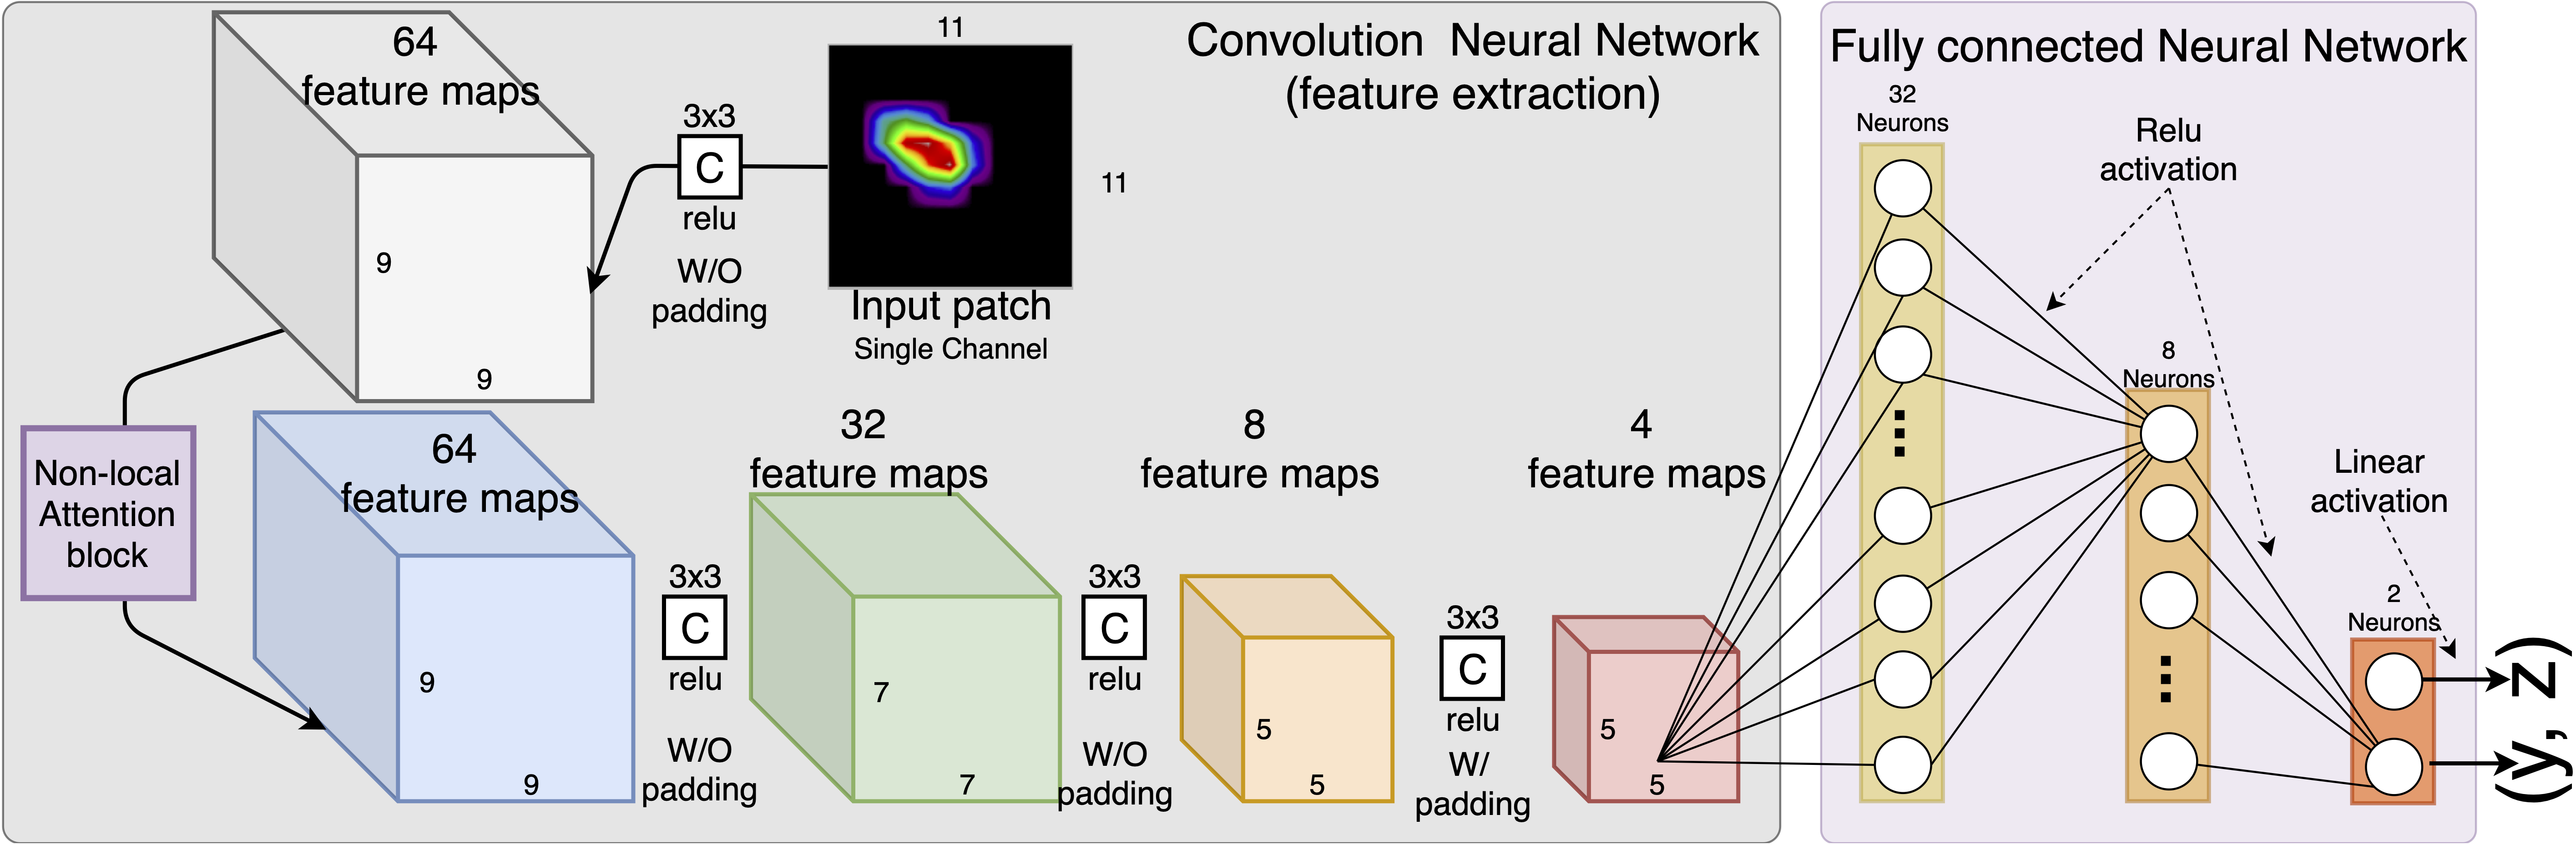
\includegraphics[width=\textwidth]{figures/BraggNN}
  \caption{This is a placeholder.}
\end{figure*}
Lowering from PyTorch to TS IR allows us to perform many useful analyses and transformations on BraggNN that would be extremely difficult (or impossible) on the original representation;
basic optimizations like dead code elimination and constant propagation are supported by TS's graph rewriting functions.
In addition, PyTorch also supports at least two kernel fusion~\cite{10.1145/2688500.2688521} tools (NNC fuser and nvfuser).
Such transformations are critical for achieving peak performance on CPUs and hardware accelerators alike but for our purposes, deployment to application specific hardware, we require a broader collection of transformations.
To this end, we turn to a recent addition to the compiler ecosystem.

\subsubsection{MLIR}\label{subsec:mlir}

Multi-level Intermediate Representation (MLIR)~\cite{https://doi.org/10.48550/arxiv.2002.11054} is a new approach to building reusable and extensible compiler infrastructure.
MLIR is composed of a set of \emph{dialect} IRs, subsets of which are mutually compatible, either outright or by way of translation/legalization.
The various dialects aim to capture and formalize the semantics of compute intensive programs at varying levels of abstraction, as well as namespace related sets of IR transformations/optimizations (called \emph{passes}).
Our entrypoint into this compiler framework is the Torch dialect~\cite{torch-mlir}, a high-fidelity mapping from TS IR to MLIR native IR, which, in addition to performing the translation to MLIR, provides for us the necessary shape refinement mentioned above.

While Torch dialect acts as a thin shim around TS IR and does little "heavy lifting", the same cannot be said for other dialects in MLIR.
For example, the linalg dialect is designed to address the hierarchical optimization problem, wherein the goal is to enable code generation of efficient code or dispatch to existing, previously optimized, kernel code, without sacrificing ease of use and performance for either path.
Practically speaking, this entails representations of common mathematical operations, such as \inlinepython{matmul}, \inlinepython{conv}, and \inlinepython{batchnorm}, explicitly declaring semantics that are traditionally obtained only through compiler analysis (such as memory dependency) and transformations on such operations completely preserving such semantics.

We make extensive use of the linalg dialect as an intermediary between lower-level dialects, such as the affine and structured control flow dialects, and Torch dialect.
The structured control flow dialect is a straightforward formalization of control flow primitives, such as conditionals and loops, so we do not discuss it in great detail.
The affine dialect, on the other hand, provides a formalization of semantics that lend themselves to polyhedral compilation techniques~\cite{polyhedral-mlir}, i.e., techniques that make dependence analysis and loop transformations efficient and reliable.

The next step in the lowering is LLVM IR, an IR that is, technically speaking, not an MLIR dialect; the purpose of further lowering to LLVM IR is to produce a representation of BraggNN that high-level synthesis tools can consume.
We Briefly discuss the role of HLS in the translation process.

\subsubsection{High-Level Synthesis and Down}\label{subsec:hlsdown}

High-level synthesis tools produce RTL descriptions of digital designs from high-level representations, such as C or C++~\cite{10.1145/2514740, ferrandi2021bambu} or LLVM IR.
In particular, Xilinx's Vitis HLS, based on the Autopilot project~\cite{Zhang2008}, recently enabled passing LLVM IR to the tool, rather than C/C++.
Given a high-level, procedural, representation, HLS performs performs three functions, in order to produce a corresponding RTL design:
\begin{enumerate}
	\item HLS schedules operations (such as \mintinline{mlir}{fmult}, \mintinline{mlir}{fadd}, \mintinline{mlir}{load}, \mintinline{mlir}{store}) in order to determine which such operations should occur during each clock-cycle. A schedule depends on three parameters:
	      \begin{itemize}
		      \item The topological ordering of the DFG/CFG of the procedural representation (i.e., the dependencies of operations on results of other operations and resources);
		      \item The completion time for each operation;
		      \item The user's desired clock rate/frequency;
	      \end{itemize}
	\item HLS associates high-level operations to particular RTL instantiations (called \emph{binding}) for those operations; for example whether to associate an add operation followed by a multiply operation to two separate digial signal processors (DSP) instances, or whether to associate them both with a single DSP instance (configured to perform fused-multiply-add);
	\item HLS builds an FSM that cycles (transitions from state to state) through the sequence of operations in the schedule.
\end{enumerate}

In addition to fulfilling these three fundamental tasks, high-level synthesis tools such as Vitis, Bambu~\cite{ferrandi2021bambu}, LegUp~\cite{10.1145/2514740} perform standard compiler optimization passes on the IR (that they either receive or produce internally).
Optimization passes such as store-load forwarding, common subexpression elimination, and constant propagation.
Loop-unrolling and tiling are also performed at the behest of the user.
Note that the scheduling problem solved by HLS is reducible an integer programming problem~\cite{tuprints9272}, instance of which are generally NP-hard.
For certain instances, the scheduling problem can be reformulated as a system of difference constraints.
Such a formulation induces a unimodular matrix representation of the constraint system which is amenable to Bellman-Ford $O(n^2 + mn)$\commnt{this is phrased poorly - unimodular guarantees you integral solutions to the LP but also gives you the shortest path analogy property}{ for checking consistency of a solution (essentially the shortest path problem) }and an LP approach for optimizing the critical path~\cite{1688836}.
Thus, ostensibly, HLS tools solve computationally intensive problems in order to produce a RTL description of a high-level representation of a DNN.
At the RTL level of abstraction, there remain two more steps prior to being able to actually deploy to an FPGA; one of them being a final lowering, so called logic synthesis, and the other being Place and Route (PnR).

Logic synthesis is the process of mapping RTL to actual hardware primitives on the FPGA (so called \emph{technology mapping}), such as lookup tables (LUTs), registers, and DSPs (in cases where they haven't been explicitly instantiated).
Logic synthesis produces a network list (netlist) describing the logical connectivity of various parts of the design.
For example,
\begin{longlisting}
	\inputminted{verilog}{sources/always.v}
	\caption[Long Code Example]{A long code example which will break across pages.}
	\label{lst:long}
\end{longlisting}
\noindent corresponds to a state of an FSM during which the registers \inlinev{reg_1608}, \inlinev{reg_1613}, \inlinev{reg_1618} are updated with new values from wires (\inlinev{fu_1076_p2}, \inlinev{notrhs18_fu_1082_p2}, \inlinev{fu_646_p2}).
Assuming these registers are updated in other FSM states (from differing wires), this logic will synthesize to multiplexers (or possibly multiplexer trees, depending on how many different input wires feed these same registers).
Such multiplexers are actually implemented using Lookup Tables (LUTs) of varying sizes and multiplcities.
Another relevant concern is the implementation of floating point operations in terms of DSPs; depending on user parameters and other design features, DSP resource consumption for floating point multiplication and addition can differ greatly.
The number of LUTs and DSPs that a high-level representation of a DNN corresponds to is relevant to both the performance and feasibility of that DNN when deployed to FPGA (more on this in Section~\ref{subsec:parallel-toposort-scheduling}).

Finally, after the netlist has been produced, the entire design undergoes PnR.
The goal of PnR is to determine which configurable logic block within an FPGA should implement each of the units of logic required by the digital design.
PnR algorithms need to minimize distances between related units of functionality (in order to minimize wire delay), balance wire density across the entire fabric of the FPGA (in order to reduce route congestion), and maximize the clock speed of the design (a function of both wire delay, logic complexity, and route congestion).
The final, routed design, can then be deployed to the FPGA by producing a proprietary \emph{bitstream}, which is written to the FPGA.

In general, both of these final steps (logic synthesis and PnR) can only be performed by the proprietary tools of the hardware manufacturers (e.g., Vivado by Xilinx) and thus, from our perspective their inner workings are completely unknown.
Recently, open source alternatives for certain FPGAs have become available, thanks to herculean efforts made to reverse engineer the various bitstream formats of, for example, some of Xilinx's architectures~\cite{6546003}, and reimplement logic synthesis and PnR in open source.
Namely, ~\cite{wolf2013yosys} is a framework for Verilog RTL synthesis and Verilog to Routing~\cite{vtr} is a framework for place and route.
% It provides a basic set of synthesis algorithms for mapping to Xilinx and Lattice FPGA (as well as ASIC standard cells).
% We use Yosys as a basis of comparison for commercial tools and as a way to investigate the limitations of those tools (i.e., when Vivado fails, we can reason by analogy with Yosys, why it might've failed).

\section{Five weird tricks accelerator manufacturers don't want you to know}\label{sec:methodology}
Inspired by the FloPoCo~\cite{8877424} project, whose floating point (FP) arithmetic core generators we employ, our design methodology can best be described as \emph{computing just right}; 
we aim for just the right amount of compute and abstraction for the task at hand, no more, no less.
This methodology stands in contrast to the design methodologies of architecture designers for commodity hardware accelerators (such as GPUs), which must support a large set of use cases.
Accordingly, our methodology consists of five techniques distilled from such general purpose architectures and tools but specialized for our specific purposes.

\subsection{Abstract Interpretation for Efficient Transformations}\label{subsec:loop-unrolling}

It is well known that the most straightforward way to achieve lowest latency inference of a DNN is to linearize the control flow graph~\cite{osti_1574050} (i.e., remove branches) and flatten the dataflow graph as much as possible~\cite{10.1145/3295500.3356173} (i.e., execute as many operations in parallel as possible).
For intermediate level representations of a DNN, this corresponds to loop unrolling followed by fusion (alternatively known as unroll and jam~\cite{thomas1971catalogue}).
For example, consider the pair of loop nests in Listing~\ref{lst:loop_fusion}, corresponding to \inlinepython{Conv2d(out_channels=64, in_channels=1, kernel=3)}.
General purpose compilers can readily unroll each of the loop nests, but prior to fusion, due to their conservative correctness guarantees, are bound to verify that memory independence constraints are satisfied for all pairs of stores and loads in each of the loop nests.
Thus, after unrolling the inner loops of the second loop nest (on \mintinline{mlir}{%i5}, \mintinline{mlir}{%i6}, \mintinline{mlir}{%i7}) we incur
\[
	\mathtt{\%c1} \times \mathtt{\%c3} \times \mathtt{\%c3} \times 2 \times 4
\]
memory independence checks.
Consequently, unroll and fuse optimizations take increasingly longer as one experiments with larger and larger unroll thresholds; the \emph{unroll threshold} determines which loops will be fully unrolled (all loops with trip count less than or equal to the threshold will be unrolled).
\begin{longlisting}
	\inputminted[highlightlines={8,9,20,21,22,25},frame=lines]{mlir}{sources/loop_fusion.mlir}
	\caption{Loop fusion and unrolling example, for loops corresponding to \inlinepython{Conv2d(64, 1, 3)}, with \hl{emphasis} on loads and stores whose independence must be verified.}
	\label{lst:loop_fusion}
\end{longlisting}
\begin{longlisting}
	\inputminted[highlightlines={5,6,11-13,16},linenos=true,frame=lines,numbersep=\mintednumbersep]{mlir}{sources/unrolled_loop.mlir}
	\caption{Unrolled and fused loop-nest, for loops corresponding to \inlinepython{Conv2d(1, 64, 3)}, with \hl{emphasis} on which store-load forwards can be performed.}
	\label{lst:storeloadforwarding}
\end{longlisting}

Following unroll and jam, we are able to perform \emph{store-load forwarding}, i.e., we are able to promote those store operations which are subsequently loaded from (with no intervening stores) to registers.
For example, consider the above fused loop nests, with the second loop nest having the inner three loops fully unrolled (see Listing~\ref{lst:storeloadforwarding}); the store operations on lines 6 and 13 can be entirely eliminated and the load operation on line 5 can be forwarded to the \inlinemlir{arith.addf} on line 15.
Note, for each load operation that follows a store operation, a compiler must check whether the store and the load access the same location in memory, and further verify that there are no intervening store operations to the same memory address.
In general, this requires solving a system of constraints~\cite{10.2307/2322281}.
We observe that as loops are further and further unrolled, the cost of this particular optimization grows polynomially; consider a fully unrolled loop nest, with many parallel dataflows, for which a store operation in one dataflow might be forwarded across a parallel dataflow (and thus incur checks against all stores and loads in that parallel dataflow).

In principle, we might rely on MLIR or LLVM to perform each of these optimization passes.
The chief impediment to relying on these general purpose compilers for our needs is the runtime complexity of the their implementations.
For arbitrary programs this development time cost moderate, especially given that most development is done without these optimization (leaving the aggressive optimizations for release builds).
For us, given that the logic and dataflow of BraggNN is fixed (having already been iterated on), and given that we are in fact searching the design space for optimal low-level representations of the DNN, the runtimes of these optimization passes are prohibitive (taking on the order of hours and sometimes even days to complete).
Moreover, often their rigor and conservatism are unnecessary given a high-level understanding of the structure of BraggNN; for example, in the case of fully unrolling the above loop nests and forwarding from the stores during initialization to the loads during accumulation, the region within which the forward is safe is clear from the semantics of convolutions.
The loop indices and corresponding memory addresses for these safe store-load forwards are simple to compute analytically and ahead of time (even in the presence of complications such as strided tensors).

In order to avoid the runtime costs associated with these conservative optimization passes, we implement an abstract interpreter for sufficiently lowered DNNs.
Concretely, we lower BraggNN to the structured control flow (\inlinemlir{scf}) dialect and then interpret this representation of BraggNN with alternative semantics.
Firstly, our interpreter evaluates functions of loop indices, such as 
\begin{minted}[autogobble,xleftmargin=0.2\columnwidth,xrightmargin=0.2\columnwidth]{mlir}
	#map = affine_map<(d0, d1) -> (d0 + d1)>
	%3 = affine.apply #map(%i3, %i6)
\end{minted}
or 
\begin{minted}[autogobble,xleftmargin=0.2\columnwidth,xrightmargin=0.2\columnwidth]{mlir}
	%3 = arith.addi %i3, %i6
\end{minted}
where \inlinemlir{%i3}, \inlinemlir{%i6} are loop indices.
This enables us to determine array indices of stores and loads, such as 
\begin{minted}[autogobble,xleftmargin=0.2\columnwidth,xrightmargin=0.2\columnwidth]{mlir}
	%2 = memref.alloca() : memref<8xf32>
	%c1 = arith.constant 1.0
	memref.store %c1, %2[%3]
\end{minted}
Note that evaluation of such memory index arithmetic is typically deferred to runtime in conventional accelerators because of either the control flow inherent in a DNN, or simply a lack of available registers (to store the results).
Thus, we are able to precompute these indices, saving cycles, because BraggNN lacks control flow and FPGAs are abundant in registers.
Note also that we do not evaluate values corresponding to \inlinemlir{memref.load}s, as they represent BraggNN weights or activations; our interpreter implements such values as proxy objects and merely records the arithmetic operations performed on them.

Secondly, our interpreter unrolls loops by executing them while enforcing SSA.
That is to say, for a loop whose body has repeated assignments to the same value (ostensibly violating SSA), such as 
\begin{minted}[autogobble,xleftmargin=0.2\columnwidth,xrightmargin=0.2\columnwidth]{mlir}
	%c0 = arith.constant 0
	%c1 = arith.constant 1
	%c3 = arith.constant 3
	%c5 = arith.constant 1.35
	scf.for %i1 = %c0 to %c3 step %c1 :
		// cast int to fp
		%2 = arith.sitofp %i1
		%3 = arith.addf %i1, %c5
\end{minted}
we execute the loop and instantiate unique identifiers for the result of each operation:
\begin{minted}[autogobble,xleftmargin=0.2\columnwidth,xrightmargin=0.2\columnwidth]{mlir}
	%c0 = arith.constant 0 
	%c1 = arith.constant 1 
	%c2 = arith.constant 2 
	%c3 = arith.constant 3 
	%c5 = arith.constant 1.35
	%2_0 = arith.sitofp %c0
	%3_0 = arith.addf %2_0, %c5
	%2_1 = arith.sitofp %c1
	%3_1 = arith.addf %2_1, %c5
	%2_2 = arith.sitofp %c2
	%3_2 = arith.addf %2_2, %c5
	%2_3 = arith.sitofp %c3
	%3_3 = arith.addf %2_3, %c5
\end{minted}
This enables us to both unroll the loop and track dataflow through arithmetic operations (see Section~\ref{subsec:parallel-toposort-scheduling}).
Finally, our interpreter reinterprets \inlinemlir{memref}s as \emph{geometric symbol tables} (i.e., symbol tables indexed by array indices rather than identifiers/names) and stores/loads as assignments/reads to/from those symbol tables.
Such semantics, in combination with fully evaluated array indices, enable us to simultaneously track dataflow through activation buffers (which appear as \inlinemlir{memref}s) and perform store/load forwarding.

The dataflow analysis carried out by our interpreter enables us to easily infer the flow of weights through the DNN and thus enables us to experiment with two weight storage strategies; namely we can either store weights as BRAMs, uniquely associated with a set of DSP blocks, or as a collection of free registers. 
The dataflow analysis also enables us to identify sequences of multiplications and additions and group them together such that they can be scheduled to reuse accumulator registers associated with floating point block instantiations (effectively forming a multiply-accumulator); 
indeed, this grouping is the chief optimization that enables us to efficiently map BraggNN to FPGA.
See Section~\ref{subsec:parallel-toposort-scheduling} for a discussion on the advantages of both of these.


% We also reinterpret remaining stores and loads to memory as reads and writes to registers, thus simplifying our design; such stores and loads would otherwise translate to stores and loads from Block RAM (BRAM).
% Furthermore, since BraggNN is a relatively small DNN, we inline absolutely all of the weight tensors as constants and perform \emph{constant propagation}.
% In summary our abstract interpreter performs the following transformations on the \inlinemlir{scf} representation of BraggNN:
% \begin{enumerate}
% 	\item We completely eliminate any latency due to loading from or storing to BRAM for intermediate activations;
% 	\item We completely eliminate all logic (i.e., integer arithmetic) related to calculating memory offsets, a non-trivial reduction in instruction count and design complexity (see figure <figure> for reduction in instruction count);
% 	\item We instantiate a reduced set of floating point operation cores, and thus reduce complexity and overall latency of our design.
% \end{enumerate}
% Note, we are able to perform the memory to registers promotions owing to the fact that BraggNN is a relatively compact DNN and our target FPGA is plentiful in registers.
% The reinterpreted semantics implemented by our abstract interpreter are presented in Eqns~\eqref{eqn:semantics}.

% \begin{figure}
% 	% \begin{equation}\label{eqn:semantics}
% 	% 	\begin{split}
% 	% 		\llbracket \%\texttt{\small var} = \inlinemlir{memref.alloca}\texttt{()}\!\!:\!\inlinemlir{memref}\!\!<\!\!k\inlinemlir{xf32}\!\!> \rrbracket &= [\text{allocate }k\text{ 16 bit registers}] \\
% 	% 		\llbracket \mintedinline{mlir}{\%5 = memref.load \%i0[\%i1, \%i5, \%3, \%4]} \rrbracket &= [\text{allocate }k\text{ 16 bit registers}] \\
% 	% 	\end{split}
% 	% \end{equation}
% 	\begin{multline*}
% 		\llbracket \inlinemlir{$\%$var = memref.alloca() : memref<$k$xf32>} \rrbracket \implies \\
% 			\text{allocate $k$ 16 bit registers}
% 	\end{multline*}
% 	\begin{multline*}
% 		\quad\llbracket \inlinemlir{$\%$5 = memref.load $\%$var[$\%$m]} \rrbracket \implies \text{read $m$th register} \quad
% 	\end{multline*}
% 	\begin{multline*}
% 		\quad\quad\llbracket \inlinemlir{$\%$8 = arith.mulf $\%$5, $\%$6} \rrbracket \implies \text{ $\%8 = \%5 \times \%6$} \quad\quad\quad
% 	\end{multline*}
% 	\begin{multline*}
% 		\quad\llbracket \inlinemlir{memref.store $\%$8, $\%$var[$\%$m]} \rrbracket \implies \text{store $\%$8 in $m$th register}\quad
% 	\end{multline*}
% 	\begin{multline*}
% 		\llbracket \inlinemlir{scf.parallel (...) = (...) to (...) step (...)} \rrbracket \implies \\
% 			 \text{store $\%$8 in $m$th register}
% 	\end{multline*}

% 	\caption{This is a placeholder.}\label{fig:semantics}
% \end{figure}

\subsection{Scheduling}\label{subsec:parallel-toposort-scheduling}

In addition to reducing the runtime of the compiler frontend, our abstract interpreter simplifies the representation such that we may emit a simplified LLVM IR to pass to downstream tools (such Vitis HLS), and thus, in theory reduce their runtime as well.
In practice, performing these optimizations has no effect on the runtime of Vitis HLS, since it reruns the same (or similar) passes as part of its transformation pipeline.
Hence, one of the first difficulties we faced in implementing BraggNN as a digital design was reducing the time taken by Vitis HLS in performing its own optimizations on the IR emitted by our interpreter. 
Furthermore, Vitis HLS' scheduling algorithms struggle with the fully unrolled representation of BraggNN (\maxx{figure with instruction counts}), due to the large number of instructions/operations.
Hence, in order to be able to quickly iterate design experiments, it became necessary to completely eliminate Vitis HLS from the design process.

Recall that one of the critical functions which Vitis HLS fulfills is the scheduling of operations during each clock cycle, in such a way that they preserve the dataflow graph of BraggNN; that schedule then informs the construction of a corresponding FSM.
As already mentioned, scheduling arbitrary programs involves formulating and solving ILP, which is an NP-hard problem.
In the resource-unconstrained case, due to the precedence relations induced by dataflow, the constraint matrix of the associated ILP is \emph{totally unimodular matrix} and the feasible region of the problem is an integral polyhedron. 
Thus, in such cases, the scheduling problem can be solved optimally in polynomial time with a (non-integer) LP solver~\cite{tuprints9272}.
While we do not find ourselves in a resource-unconstrained environment, we are still able to make use of this fact by studying the structure of BraggNN.

%  by imposing dependencies on operations that model a fixed number of resources.
Consider again the second loop in Listing~\ref{lst:loop_fusion}, which corresponds to the first convolutional layer of BraggNN.
If we rewrite it using pseudocode
\inputminted[autogobble,xleftmargin=0.0\columnwidth,xrightmargin=0.0\columnwidth]{mlir}{sources/loop_fusion_mac.mlir}
\noindent it is easy to observe that the loop can be parallelized on indices \inlinemlir{%i1, %i2, %i3, %i4}.
Furthermore, it can be observed that inner three loops (on indices \inlinemlir{%i5, %i6, %i7}) represent multiplication and accumulation into \inlinemlir{%tmp}.
Hence, this loop nest can be implemented as 
\[
	\mathtt{\%c1} \times \mathtt{\%c64} \times \mathtt{\%c9} \times \mathtt{\%c9}
\]
\emph{processing elements} (PE) operating in parallel, where each PE performs \inlinemlir{mulf} and \inlinemlir{addf} in parallel (the \inlinemlir{addf} operates on the results of the \inlinemlir{mulf} from the previous iteration).
Note that this structure is replicated for all convolutional layers in BraggNN.
Thus, our interpreter records this implicit parallelism (by interpreting \inlinemlir{scf.parallel} loop nests) and uses it to create auxiliary dependencies between operations (in addition to dataflow dependencies).
For example, the above loop nest is interpreted as 
\inputminted[autogobble,xleftmargin=0.0\columnwidth,xrightmargin=0.0\columnwidth]{mlir}{sources/loop_fusion_parallel.mlir}
\noindent and unrolls to 
\inputminted[autogobble,xleftmargin=0.1\columnwidth,xrightmargin=0.1\columnwidth]{mlir}{sources/loop_fusion_parallel_unroll.mlir}
\noindent where the pairing of dataflow dependency (i.e., SSA values like \inlinemlir{%44}) and \inlinemlir{pe} constrain the scheduling of the arithmetic operations.
Note that this PE dependency naturally captures the implicit geometry of the operations as well and thus, in principle, minimizes data movement between the PEs (see Section~\ref{sec:discussion} for more on this).
We can similarly constrain the other operations in BraggNN (such as \inlinemlir{relu}).
Using the complete set of constraints we formulate the resource-unconstrained problem and solve it using a LP solver (Gurobi through OR-Tools through CIRCT~\cite{CIRCTHardwareDesign}).

The behavior of our interpreter with respect to two subtleties merits discussion: fan-out from a particular PE at interface of two DNN layers and the evaluation order of \inlinepython{nn.Softmax}.
With respect to the former, consider consecutive convolutions
\begin{longlisting}
	\inputminted[frame=lines]{mlir}{sources/consecutive_convs.mlir}
	\caption{Consecutive convolutions illustrating high-fanout from \mintinline{mlir}{\%tmp}.}
	\label{lst:consecutive_convs}
\end{longlisting}
With respect to fan-out from a particular PE, since, by grouping multiplies and accumulates we enforce reuse of result registers, we produce instances of high-fanout from PE result registers at the points \emph{between DNN layers}.
Consider the consecutive convolutions in Listing~\ref{lst:consecutive_convs}; the result registers of each PE (corresponding to \mintinline{mlir}{%tmp}) have a fan-out of $64 \times k$, where $k$ is the number of other convolutions operating on \mintinline{mlir}{%tmp} (occurring in parallel). 
More importantly those 64 reads happen sequentially, and thus if the source PE participates in the evaluation of the second convolution (i.e., its result register is overwritten), the computed value will be wrong (essentially a write-after-read error).
The solution is to reuse result registers of PEs during the evaluation of a layer (saving registers) and copy results to intermediate registers \emph{between layers}. 
We handle this by enforcing value semantics at the PyTorch level of abstraction (i.e., we insert tensor copies on outputs).
With respect to the evaluation order of \inlinepython{nn.Softmax}, consider the naive implementation involves elementwise \inlinemlir{expf} followed by sum. 
Evaluating the sum sequentially is clearly wasteful (in terms of latency) and unnecessary; the solution is to enforce the instantiation of a reduction tree of adjacent sums.
Our interpreter implements this (as a \inlinepython{ReduceAdd} operation) and such a reduction tree collapses the latency logarithmically.

\subsection{Bit Twiddling Hacks}\label{subsec:bit-twiddling-hacks}
\maxx{just btw this is not a term i invented... \url{https://graphics.stanford.edu/~seander/bithacks.html}}

FPGAs do not effectively permit dynamic reconfiguration of DSPs, to support fully distinct operations; e.g., a set of DSPs associated with floating point addition can be dynamically reconfigured to perform subtraction but multiplication (likewise vice-versa).
Thus, in order to maximize reuse of DSPs (in order to minimize DSPs consumption) we only instantiate FP cores for multiplication and addition.
We use FloPoCo~\cite{8877424} core generator to generate pipelined implementations of FP addition and multiplication\footnote{FloPoCo's floating point format differs slightly from IEEE754, foregoing subnormals and differently encoding zeroes, infinities and NaNs, for the benefit of reduced complexity.}.
We map the remaining operations in BraggNN (\inlinemlir{subf}, \inlinemlir{expf}, \inlinemlir{relu}, \inlinemlir{divf}) to \inlinemlir{mulf} and addition \inlinemlir{addf}.
For the cases of \inlinemlir{subf} and \inlinemlir{expf} this is straightforward (a bit flip on the sign bit to handle the former and a Taylor series expansion to handle the latter).
For the case of \inlinemlir{relu}, note that for a IEEE 754 $n$-bit floating point number $x$
$$
\max(0, x) = x \iff x[0] = 0
$$
where $x[0]$ represents the sign bit of $x$.
A similar relationship holds for FloPoCo FP format.
Division, needed for implementing \inlinepython{nn.Softmax}, is the only primitive operation that presents a serious challenge to normalization in this way (i.e., a mapping in terms of multiplication and addition).
To represent division (in terms of \inlinemlir{mulf}) we exploit the fact that aliasing a floating point number as an integer effectively calculates the approximate binary logarithm~\cite{enwiki:1081681080} of the number.
To see this, observe that for $x=2^{e_{x}}(1+m_{x})$ it's the case that
\[
	\log _{2}(x)=e_{x}+\log _{2}(1+m_{x})	\approx e_{x} + m_x + \sigma
\]
where $\sigma$ is a free parameter used to fit the approximation.
Taking $I_x$ to be the bits of floating point $x$ interpreted as an integer, we have 
\[
\begin{aligned}
	I_{x}&=E_{x}L+M_{x}\\
	&=L(e_{x}+B+m_{x})\\
	&=L(e_{x}+m_{x}+\sigma +B-\sigma )\\
	&\approx L\log _{2}(x)+L(B-\sigma )
\end{aligned}
\]
where $E_{x}$ is the "biased exponent" ($e_x + B, B = 127$), $L = 2^{23}$, $M_{x}=m_{x}\times L$.
Thus, if $y = 1/x$, approximating both $\log y$ and $\log x$, we have 
\[
	{\frac {I_{y}}{L}}-(B-\sigma )\approx -\left({\frac {I_{x}}{L}}-(B-\sigma )\right)	
\]
or
\[
	I_{y}\approx 2 L(B-\sigma ) - I_{x}
\]
which, when taking $\sigma \approx 0.0450466$ can be expressed as 
\[
	I_y \approx \texttt{0x3F7A3BEA} - I_x
\]
thus reducing division to the composition of subtraction (or addition of the negative) and multiplication.
In our experiments (and prior work~\cite{10.1007/978-0-387-72258-0_14}) this approximation incurs approximately a $4\%$ difference in accuracy per division.

Finally, we experiment with alternative bitwidth implementations of floating point.
With respect to the BraggNN training, we observe that the sample data does not use a full 8 bit exponent (see Figure~\ref{fig:numexp}).
\begin{figure}
	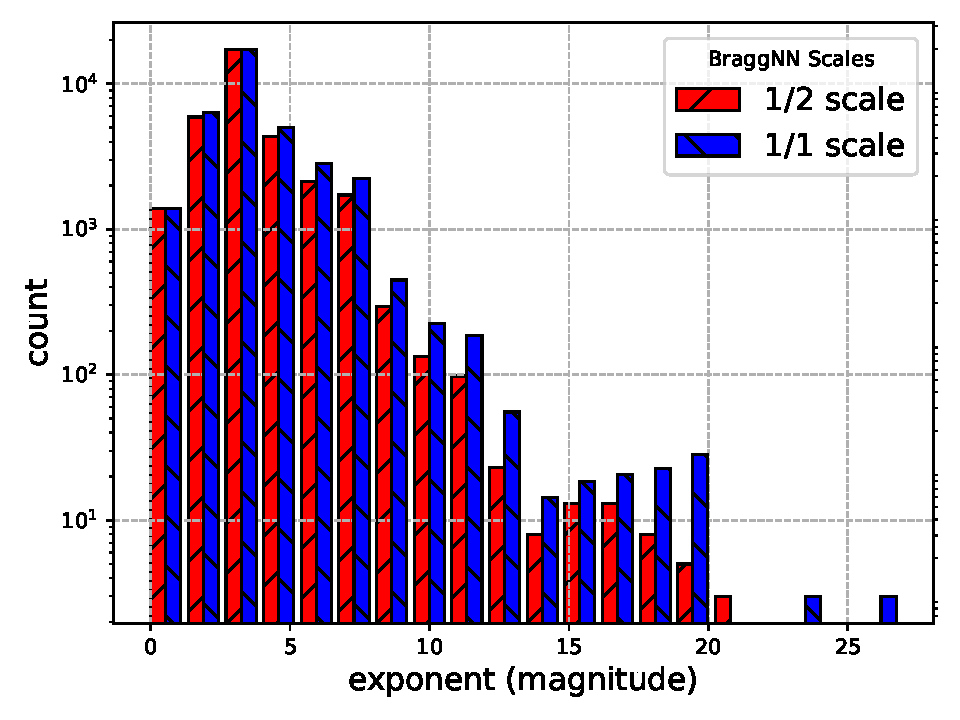
\includegraphics[width=\columnwidth]{figures/exp_hist}
	\caption{Range of exponent values for BraggNN weights.}\label{fig:numexp}
\end{figure}
With this in mind, we deploy BraggNN using quarter precision floats, i.e., using 4 bits to represent the exponent and 4 bits to represent the mantissa.
There is ample prior that shows 8-bit floating point is adequate during training and inference~\cite{https://doi.org/10.48550/arxiv.1812.08011, https://doi.org/10.48550/arxiv.2206.02915, https://doi.org/10.48550/arxiv.2001.05674}.
This produces floating point arithmetic cores that use fewer registers, LUTs, and having smaller wire delays, again leading to a reduction in overall complexity and end to end latency.


\section{Evaluation}\label{sec:evaluation}
We evaluate our design methodology, as applied to BraggNN, and a few NN functional units, against ScaleHLS\cite{ye2021scalehls} and SODA-OPT\cite{9516615}, two state-of-the-art but general purpose DNN compiler to HLS tool flows.
Both tools perform design space exploration but at the cost of high-runtimes and ultimately inferior results \emph{when latency is the only metric}.


\begin{figure}
	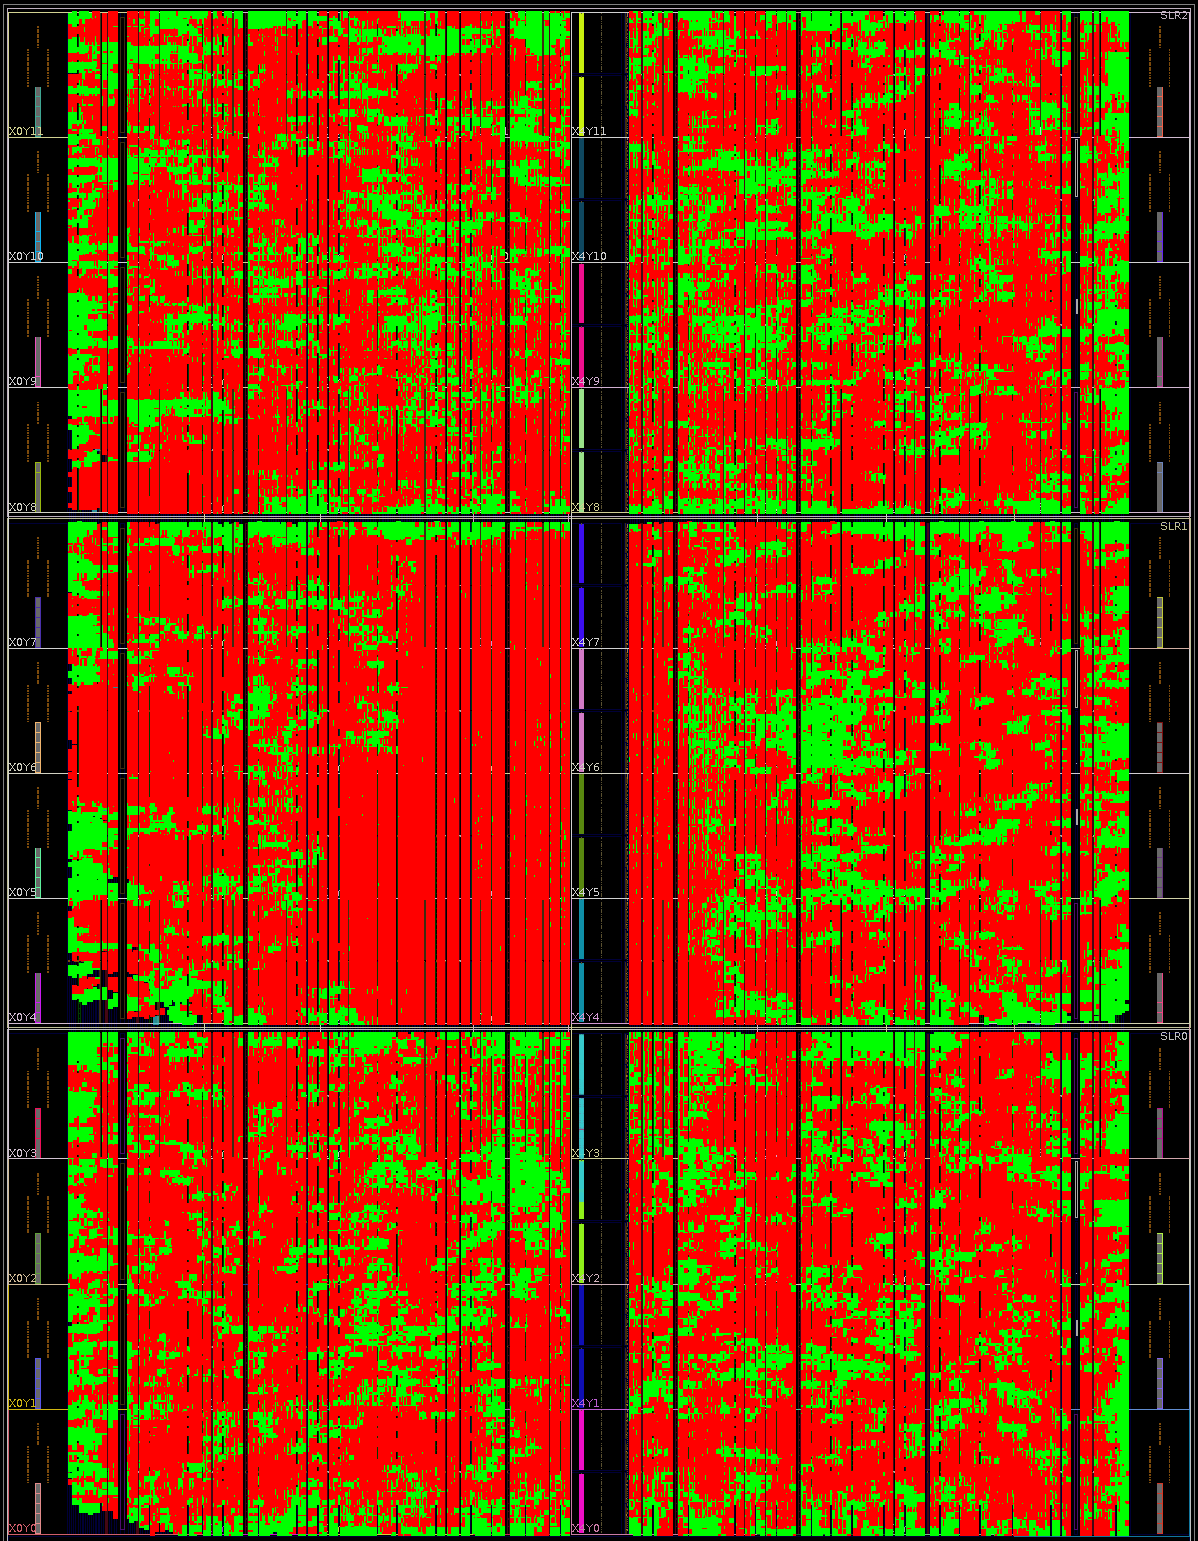
\includegraphics[width=\columnwidth]{figures/fp16_placed}
	\caption{Fully synthesized and placed \emph{but not routed} (on Xilinx Alveo U280) design for BraggNN with IEEE754 FP16. \crule[red]{0.25cm}{0.25cm} regions represent \texttt{fmul} leaf cells, while \crule[green]{0.25cm}{0.25cm} regions represent \texttt{fadd} leaf cells.}\label{fig:placed_braggnn}
\end{figure}

\begin{figure}
	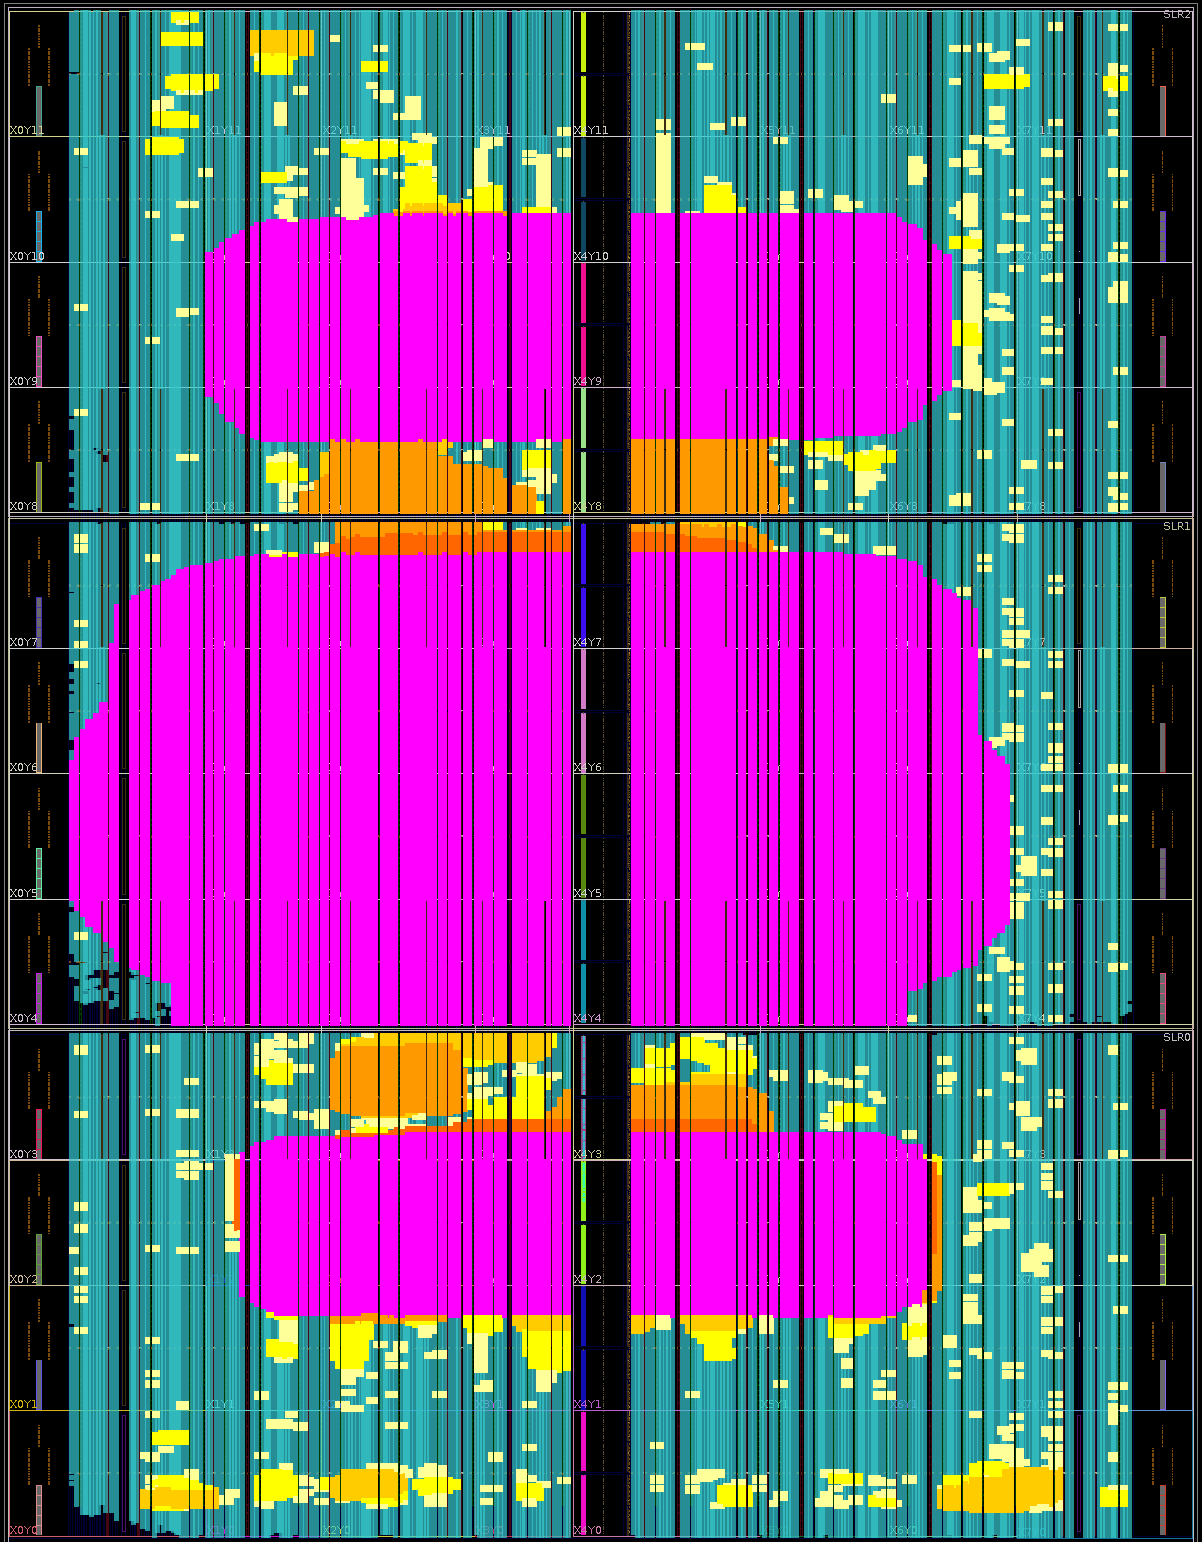
\includegraphics[width=\columnwidth]{figures/alveo_congestion}
	\caption{Fully synthesized and placed \emph{but not routed} (on Xilinx Alveo U280) design for BraggNN IEEE754 FP16. \crule[magenta]{0.25cm}{0.25cm} regions represent areas of high congestion, while \crule[orange]{0.25cm}{0.25cm} and \crule[yellow]{0.25cm}{0.25cm} regions represent areas of moderate (\crule[teal]{0.25cm}{0.25cm} regions represent negligible congestion).}\label{fig:congestion_alveo}
\end{figure}

\begin{figure}
	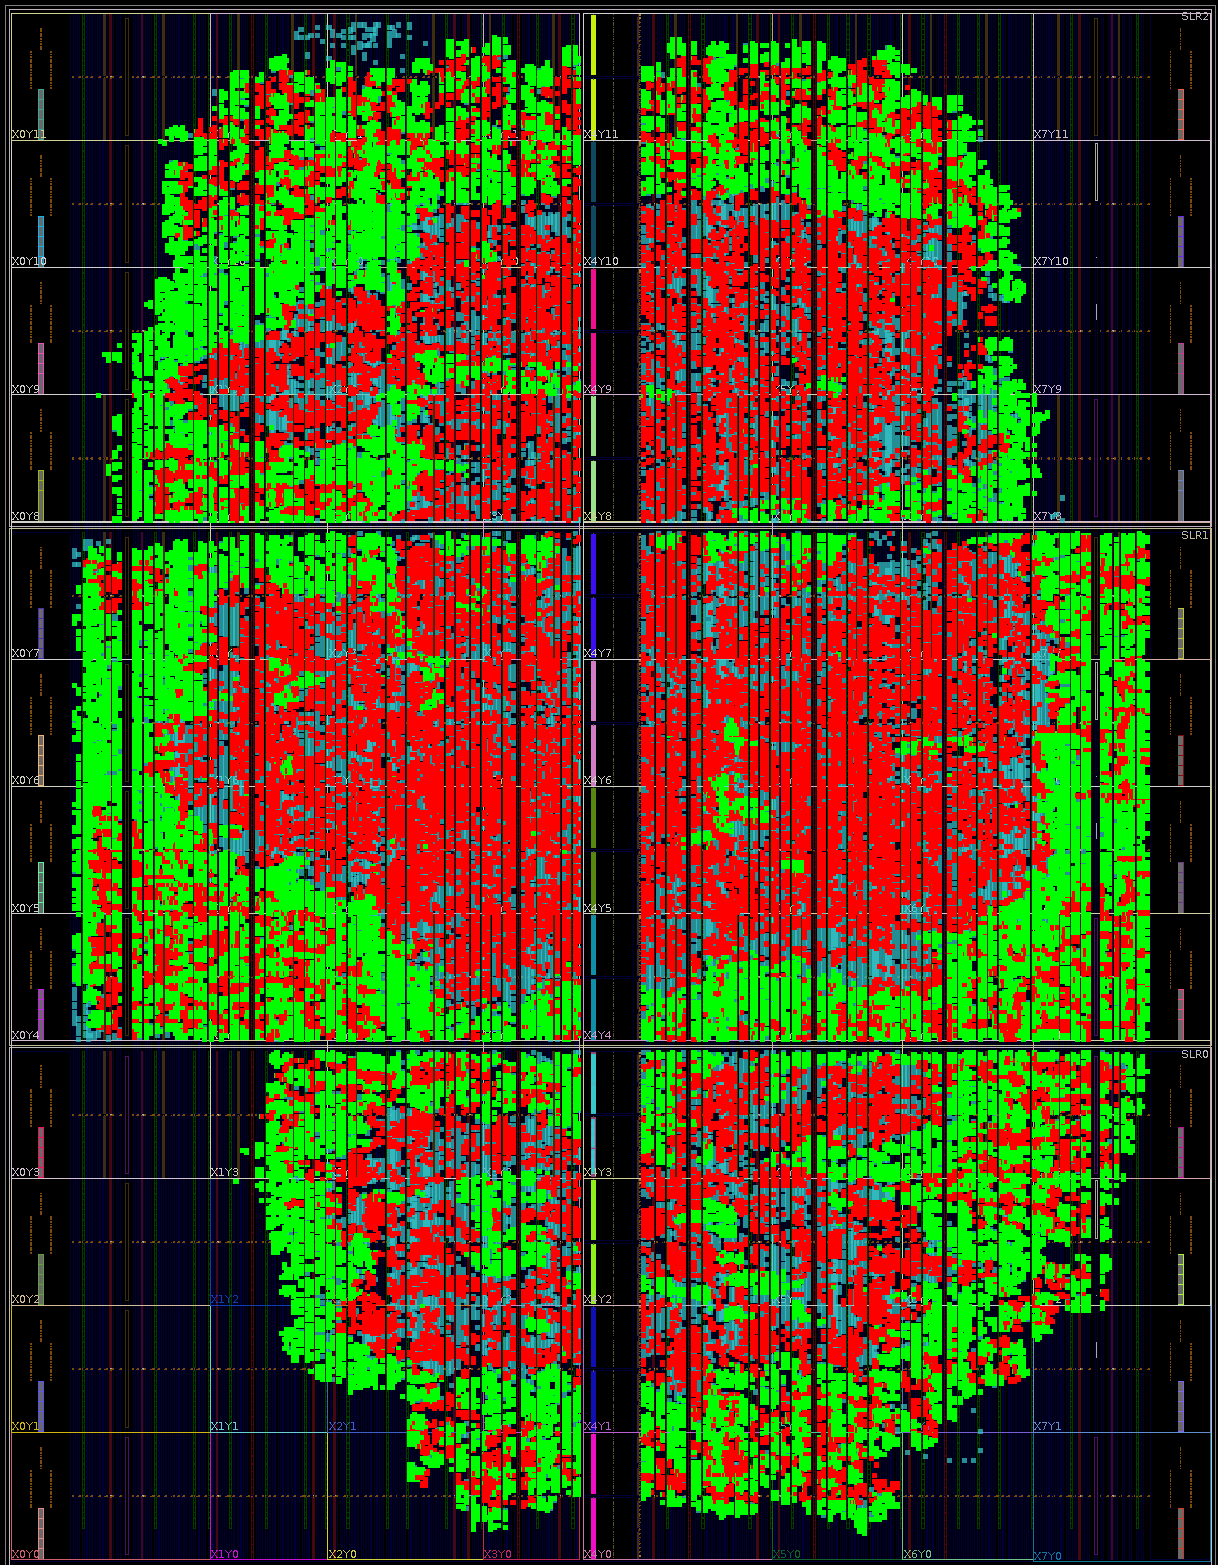
\includegraphics[width=\columnwidth]{figures/correct_schedule_routed}
	\caption{Fully synthesized, placed, \emph{and routed} (on Xilinx Alveo U280) design for BraggNN with FloPoCo FP8. \crule[red]{0.25cm}{0.25cm} regions represent \texttt{fmul} leaf cells, while \crule[green]{0.25cm}{0.25cm} regions represent \texttt{fadd} leaf cells.}\label{fig:placed_braggnn}
\end{figure}

\begin{figure}
	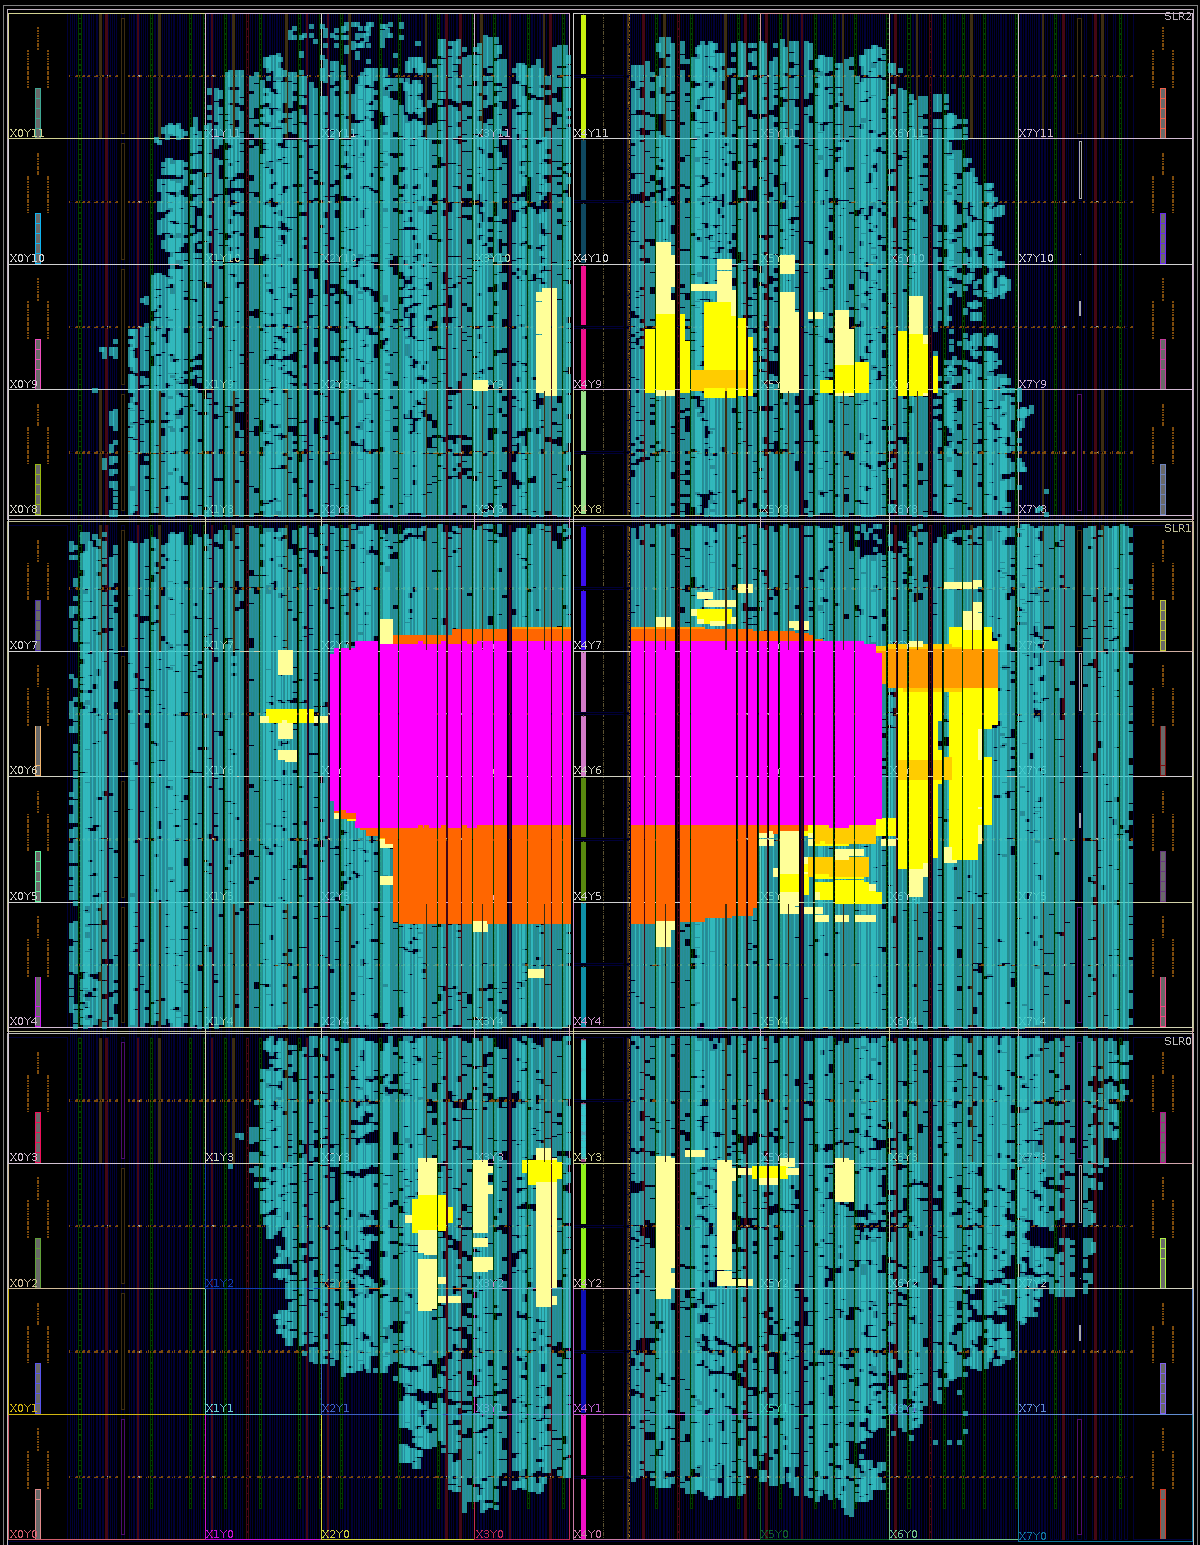
\includegraphics[width=\columnwidth]{figures/sfp_congestion.png}
	\caption{Fully synthesized, placed, \emph{and routed} (on Xilinx Alveo U280) design for BraggNN with FloPoCo FP8. \crule[magenta]{0.25cm}{0.25cm} regions represent areas of high congestion, while \crule[orange]{0.25cm}{0.25cm} and \crule[yellow]{0.25cm}{0.25cm} regions represent areas of moderate (\crule[teal]{0.25cm}{0.25cm} regions represent negligible congestion).}\label{fig:congestion_alveo}
\end{figure}

\section{Acknowledgements}

\bibliographystyle{ACM-Reference-Format}
\bibliography{ref}


\end{document}
